
% {{{ preamble

\documentclass{article}

\usepackage{url}
\usepackage{hyperref}
\usepackage{graphicx}
\usepackage{nonfloat}
\usepackage{amsmath}
\usepackage{fancyvrb}
\usepackage{parskip}
\usepackage{verbatimbox}
\usepackage{color}

\usepackage{courier}
\usepackage{listings}
\lstset{numbers=left,
		language=C,
		tabsize=4,
		basicstyle=\ttfamily,
		columns=fixed,
		%basicstyle=\footnotesize,
		showstringspaces=false,  % don't show the space character
		%commentstyle=\textit,
		showtabs=false,
		extendedchars=true,
		basicstyle=\normalsize,
		captionpos=b,
		frame=tb,
		xleftmargin=0.3in}

\usepackage{vmargin}  % make the margins a bit smaller
%\setmarginsrb{1.0in}{1.0in}{1.0in}{1.0in}{0in}{0.4in}{0.0in}{0.40in}
\setmarginsrb{1.0in}{1.0in}{1.0in}{1.0in}{0in}{0.25in}{0in}{0.20in}

\raggedright

\usepackage[backend=biber,autocite=footnote,
			bibstyle=authortitle,citestyle=verbose-inote]{biblatex}
\setlength{\bibitemsep}{\baselineskip}

\addbibresource{references.bib}

\graphicspath{{figs/}}
% }}}

\begin{document}

\VerbatimFootnotes

% {{{ title page

\thispagestyle{empty}

\centerline{\Large \textbf{SprinklerPI}}
\vspace{0.1in}
\centerline{\normalsize {Jeremiah Mahler} ({\href{mailto:jmmahler@gmail.com}{jmmahler@gmail.com}})}
\centerline{\small \today}
\vspace{0.2in}

% }}}

%\tableofcontents
%\pagebreak

% {{{ Introduction
\section{Introduction}

The task of watering your lawn is conceptually simple.
Turn on certain sprinklers at certain times and run them for
a certain duration.

The well known UNIX/Linux program \verb+cron+ can run any program
on any schedule: every day, every other day, every third Friday,
every day during the month of august.  The possible combinations
are endless.

Using the power of \verb+cron+ on a RasberryPI\autocite{rasberrypi}
running Linux with a small amount interface hardware to control the
sprinkler valves and the result is a very powerful sprinkler control system.

% }}}

\clearpage
\section{Control}
\label{sec:control}

Before the sprinkler valve can be driven, some control logic is necessary
between the RasberryPI and the driver (Section \ref{sec:driver}).
Most residential sprinkler systems are capable of driving eight circuits.
And only one of these circuits can be active at any one time
\footnote{If multiple circuits were active this could lower the
water pressure resulting in inconsistent watering amounts.}.
This controller uses the same design
\footnote{With some minor redesign this controller could be
expanded to control a large number of circuits possibly
with multiple active circuits at a time.}.

The RasberryPI has enough GPIO pins to control each valve independently.
But doing this would be a waste.
Future expansion to a large number of circuits would be severely limited.
And the time requirements are very generous.
Being able to switch a valve every second is more than adequate.

Instead of using individual GPIO pins, the four SPI pins provided by
the SPI are used.
This design sends 8-bits for each message (Figure \ref{fig:spi}).
But only three bits are used to address each valve ($2^3 = 8$).
If the design was simply expanded to use the available bits
it could address 128 valves ($2^7 = 128$).

\begin{verbbox}
  7      4 3      1      0
 +--------+--------+------+
 | unused | valve# | en_n |
 +--------+--------+------+
\end{verbbox}
\begin{figure}[hbp]
\centering
\theverbbox
\caption{SPI message format.}
\label{fig:spi}
\end{figure}

Going from SPI to signals which can turn on/off a valve requires
more logic than has been discussed so far.
A shift register is needed to take the bits as inputs.
A decoder is needed to convert shifted in number to a single
bit output.
And in this case, since the 74LS138 decoder is used, the outputs
must be inverted.
Figure \ref{fig:control} shows the control schematic.

\begin{figure}[hbp]
% TODO
\caption{Sprinkler valve control logic.}\label{fig:control}
\end{figure}

\clearpage
\section{Driver}
\label{sec:driver}

\begin{figure}[hbp]
\centering
%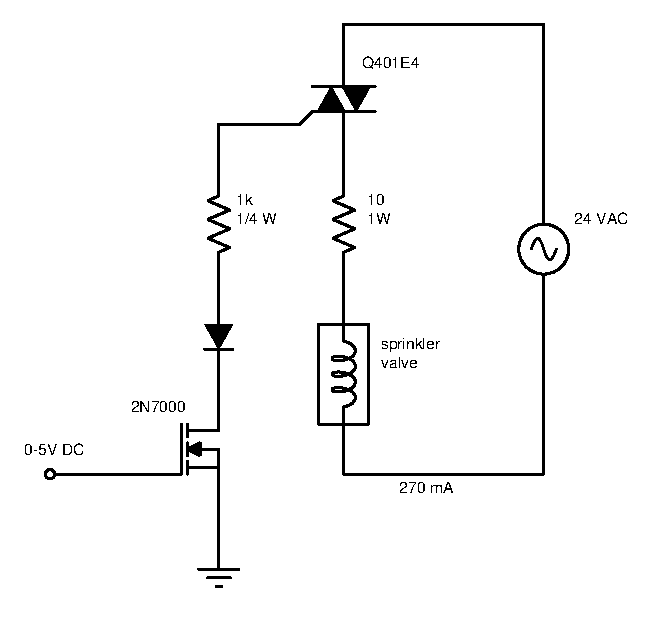
\includegraphics[scale=1.5]{figs/driver}
\def\svgwidth{270px}
\input{figs/driver.pdf_tex}
\caption{Sprinkler valve driver circuit.}\label{fig:driver}
\end{figure}

To turn the sprinkler valves on and off requires 24 VAC
and approximately 270 mA.
If it is assumed that during steady state both the solenoid
and the triac have negligible resistance (Figure \ref{fig:driver}),
a 10 $\Omega$ resistor can be used to limit the current to 240 mA.

The control signal to the triac (Q401E4) is very sensitive.
The tinyest current will cause it to conduct.
If it is driven by a 0-5V signal it will conduct not only
with a 5V signal but also with 0V signal.
To overcome this issue a diode was used to ensure no current
flows when it is reverse biased.
The FET (2N7000) is used to switch the triac while it also
serves to limit the control current of a 0-5 volt signal
to less than 0.5 mA.
This current draw is then well within the limits typical CMOS logic.

\pagebreak
\printbibliography

\end{document}
